\chapter*{Johdanto}

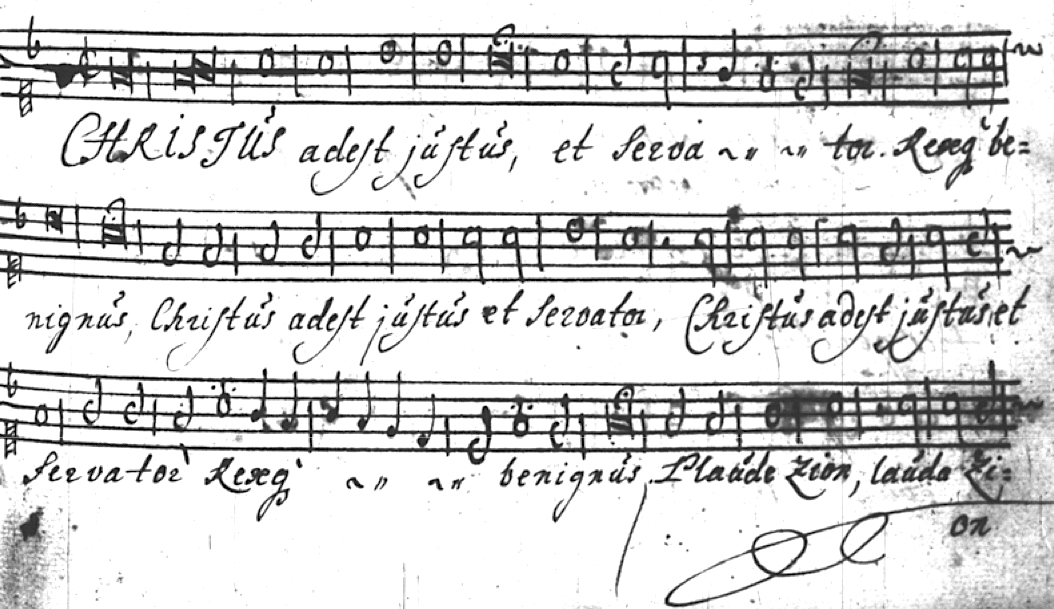
\includegraphics[scale=0.45]{../facsimile/christus-adest-justus}

1600- ja 1700-luvuilla Suomessa ei ollut rikkaita hoveja suurine muusikkokuntineen. Musiikkielämä ei silti rajoittunut kansanmusiikkiin. Myös oppinutta musiikkia harrastettiin kirkkojen, koulujen, kaupunginpuhaltajien ja sotilassoittokuntien piireissä. Suurimmissa kaupungeissa kuten Turussa, Porissa, Vaasassa ja Viipurissa nämä tahot kykenivät yhdistämään voimansa ja esittämään moniäänistä, jopa monikuoroista musiikkia kirkollisissa ja muissa juhlissa.

Vielä tuohon aikaan musiikki oli tärkeä osa luterilaisten maiden koulusivistystä. Itämeren alueella olikin erityinen, melko yhtenevä koulumusiikkiohjelmisto, johon tutustuminen korjaa sitä yleistä virhekäsitystä, että entisaikaan olisi esitetty vain uutta musiikkia. Suosituinta koulumusiikkia eivät suinkaan olleet ajan tunnetuimpien säveltäjien uudenaikaisimmat luomukset, vaan 1500-luvun ja 1600-luvun alun vokaalipolyfonia. Vanhakantaisuus ei ollut osoitus Pohjolan taantumuksellisuudesta, sillä samaa perinteistä ohjelmistoa käytti myös esimerkiksi Bach Leipzigissä.

Tärkein, joskin edelleen huonosti tunnettu todistus Suomessa harjoitetusta koulumusiikista ovat Porin triviaalikoulun nuottikirjat, jotka Heikki Klemetti löysi Porin Lyseon kirjastosta yli sata vuotta sitten. Nämä neljä äänikirjaa on kopioitu käsin vuonna 1725 triviaalikoulun käyttöön, mahdollisesti korvaamaan isovihan aikana hävitettyjä aiempia nuottikirjoja, ja ne sisältävät 4-, 5- ja 8-äänistä hengellistä vokaalimusiikkia. Kokoelman 93 sävellystä ovat latinan- ja ruotsinkielisiä. Vain yksi, Melchior Vulpiuksen Matteus-passio vuodelta 1613, on suomeksi käännetty. Sama teos on säilynyt lukuisissa muissakin suomalaisissa lähteissä ja sillä oli Suomessa yli sata vuotta yhtäjaksoisesti kestänyt esitysperinne.

Vulpiuksen passio on myös ainoa Porin nuottikirjoihin sisältyvä teos, jonka säveltäjä on nimeltä mainittu. Äänikirjojen kopioija ei nähtävästi pitänyt säveltäjätietoja tärkeinä, eikä montaakaan kappaleen säveltäjää ole vielä kyetty nimeämään. Lukuisat venetsialaistyyliset kaksoiskuoromotetit ovat tunnistettavissa slovenialaissyntyisen Jacobus Galluksen teoksiksi. Galluksen musiikkia on runsaasti myös kuuluisassa Florilegium Portense -kokoelmassa, jota myös Bach käytti. Toinen Suomessa suosittu koulusäveltäjä oli Rostockin urkuri Daniel Friderici, jonka sävellyksiä on myös Piae Cantiones -kokoelman vuoden 1625 painoksessa.

Eräät nuottikirjojen sävellykset ovat vanhoja populaarisävelmiä, joihin on sepitetty uusi, hengellinen teksti. Nunc zymphonizate on alun perin Giovanni Gastoldin balletto La sirena. Christus factus est pro nobis taas on alkujaan instrumentaalinen pavana La Bataille, joka puolestaan lainaa Clément Janequinin samannimistä chansonia vuodelta 1515. Susanna se videns kertoo olennaisimman osan Vanhan Testamentin apokryfikirjoihin sisältyvästä Susannan ja vanhimpien tarinasta, joka tunnettiin eri puolilla Eurooppaa Orlando di Lasson viisiäänisenä, runsaan polyfonisena madrigaalina. Porin nuottikirjoihin on kuitenkin valittu Didier Lupin yksinkertainen neliääninen versio. Tämä ratkaisu on luonteenomaista koulumusiikkikokoelmille, joissa tarkoituksella vältettiin monimutkaista polyfoniaa. Silti monet Porin äänikirjoihin sisältyvät sävellykset ovat taitavasti tehtyjä ja musiikillisesti vaikuttavia. Eräät äänenkuljetuksellisesti kömpelöt kappaleet saattavat olla paikallisten muusikoitten työtä jommalta kummalta puolen Pohjanlahtea.



\textit{Teksti: Jaakko Saarinen}
